\documentclass{skript}

\title{Traveling Salesman Problem}
\lecturer{Prof.\ Dr.\ Jens Vygen}
\author{Nicholas Schwab}
\date{Winter Term 2019/20}
\tikzset{every picture/.style={line width=2pt}}
\tikzset{graph node/.style={circle,minimum width=4pt, fill, inner sep=0pt, black}}


\newcommand{\kant}{to node[at start, graph node]{}}



\bibliography{literature}

\begin{document}
\thispagestyle{plain}
These notes are on the Advanced Topics lecture on the Traveling Salesman Problem in the winter term 2019/20 at the University Bonn.

\tableofcontents

\chapter{Introduction}
There are no formal prerequisites for this lecture.
There should be a grounding in combinatorial optimization, linear programming and graph theory.
The oral exam will likely take place on February 11th.

\begin{definition}[Symmetric Traveling Salesman Problem]
    An instance of the symmetric \emph{Traveling Salesman Problem} consists of a finite set $V$ of cities and symmetric distances $v(v,w) \geq 0$ for all $v,w\in V$.
    The task is to find a finite sequence $v_0,v_1, \dots, v_k\in V$ such that
    \begin{itemize}
        \item 
            every city appears at least once,
        \item 
            $v_0 = v_k$
    \end{itemize}
    minimizing $\sum_{i=1}^k c(v_{i-1}, v_i)$.
\end{definition}

This is equivalent to a better known variant, where each city is visited exactly once and the distance function is required to fulfill the triangle inequality.

\begin{lemma}
    Both variants are equivalent.
\end{lemma}
\begin{proof}
    \begin{description}
        \item{Reduction from 1 to 2:} Compute the metric closure of the complete graph on $V$.
    So $\tau(v,w) \coloneqq \min\left\{C(E(P)) \such P \text{ is a } v-w-\text{path}\right\}$. 
    Now solve the instance of the second instance, since $\tau$ fulfills the triangle inequality. 
    We then replace each edge by a path of the same cost which gives a solution of the first variant with the same costs.
\item{Reduction from 2 to 1:} We solve the TSP possibly visiting nodes more then once.
    Then we visit the nodes in order skipping every node we already visited.
    Due to the triangle inequality this can not increase the cost of the solution.
    \end{description}
\end{proof}

\begin{definition}[Tour]
    Instead of a sequence of nodes we may ask for a multi-set $F$, called a \emph{tour} of edges such that $(V,F)$ is connected and $(V,F)$ is Eulerian (i.e., every vertex has even degree).
    This is a third version of the TSP and often it is the most useful version.
\end{definition}

\begin{definition}[Graph TSP]
    The \emph{graph TSP} is a special case of the symmetric TSP.
    On a given undirected graph $G$, find a tour $F$ in $G$, so a multi-subset of $E(G)$, minimizing $|F|$.
    Since we can define $c(v,w) = \dist_g(v,w)$ this is indeed a special case of TSP.
\end{definition}

\begin{figure}
    \centering
    \begin{minipage}[b][3.3cm]{.4\textwidth}
        \centering
    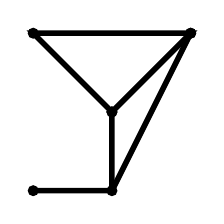
\begin{tikzpicture}
        \draw (0,0) \kant (1,0) \kant (1,1) \kant (0,2) \kant (2,2) \kant (1,1) node[graph node]{};
        \draw (2,2) \kant (1,0);
    \end{tikzpicture}
    \vfill
    \caption{A graph}
    \end{minipage}\qquad
    \begin{minipage}[b][3.3cm]{.4\textwidth}
        \centering
    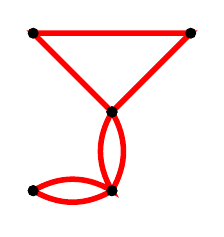
\begin{tikzpicture}
        \draw[red] (4,0) [bend right] \kant  (5,0) \kant (5,1);
        \draw[red] (5,1)\kant (4,2) \kant (6,2) \kant (5,1)node[graph node]{};
        \draw[red] (4,0)[bend left] \kant (5,0) \kant (5,1)node[graph node]{};
    \end{tikzpicture}
    \vfill
    \caption{Minimum tour}
    \end{minipage}
    \ \vspace{10pt} 

    \begin{minipage}[b][3.3cm]{.4\textwidth}
        \centering
    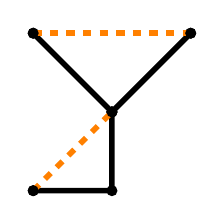
\begin{tikzpicture}
        \draw (0,0) \kant (1,0) \kant (1,1) \kant (0,2) node[graph node]{};
        \draw (2,2) \kant (1,1)node[graph node]{};
        \draw[orange, dashed] (0,0) \kant (1,1)node[graph node]{};
        \draw[orange, dashed] (0,2) \kant (2,2)node[graph node]{};
    \end{tikzpicture}
    \vfill
    \caption{MST and matching}
    \end{minipage}\qquad 
    \begin{minipage}[b][3.3cm]{.4\textwidth}
        \centering
    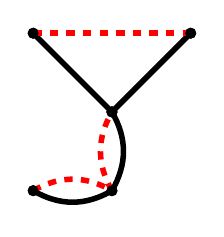
\begin{tikzpicture}
        \draw (0,0)[bend right] \kant (1,0) \kant (1,1);
        \draw (1,1) \kant (0,2) node[graph node]{};
        \draw (2,2) \kant (1,1)node[graph node]{};
        \draw[red, dashed] (0,0) [bend left]\kant (1,0) \kant (1,1)node[graph node]{};
        \draw[red, dashed] (0,2) \kant (2,2)node[graph node]{};
    \end{tikzpicture}
    \vfill 
    \caption{MST and $T$-Join}
    \end{minipage}
\end{figure}

\begin{algo}[$2-$approximation for graph TSP]\label{alg:doubletree}
    Compute a minimum spanning tree $(V,S)$ for $G$ and output $2S$, the multi-set of all edges of $S$ taken twice.
\end{algo}

\begin{algo}[$\frac32-$approximation, (Christofides 1976, Serdjukov 1978)]\label{alg:christofides}
    We first again compute a MST $(V,S)$.
    Let $\odd(S) \coloneqq \left\{v\in V\such |\delta_S(v)| \text{ is odd}\right\}$.
    In the metric closure: Find a min-weight perfect matching $M$ in the complete graph on $\odd(S)$.
    Alternatively, let $T=\coloneqq \odd(S)$ and compute a min-weight $T$-join $J$. 
    Output $S\cup J$.
\end{algo}

\begin{definition}[$T$-Join]
    Given a graph $G$ and some $T\subseteq V(G)$ with $|T|$ even.
    A \emph{$T$-join} is a set $J\subseteq E(G)$ such that $\odd(J) = T$.
\end{definition}

\begin{thm}\label{thm:christofides}
    Algorithm~\ref{alg:christofides} is a $\frac32-$approximation algorithm.
\end{thm}
\begin{proof}
    Let $\OPT$ be the cost of an optimal tour.
    The cost of $S$ is at most $\OPT$ since $\OPT$ contains a spanning tree.
    Given an optimum tour, we can partition it in two $T-$joins, for every $T\subseteq V$ with $|T|$ even. 
    For this we color the tour red and blue, changing colours whenever we visit a city for the first time.
\end{proof}

\begin{note}
    If we want to visit each node exactly once but do not have the triangle inequality on the cost function, approximating an optimal solution up to a constant factor is NP-hard.
    Assuming we had an $k$-factor algorithm, we could take an instance of the Hamilton-Path-Problem and add all edges missing from the complete graph with weight $nk+1$.
    Then the $k$-factor algorithm finds a solution of weight smaller then $nk$ if and only if there is a Hamilton-Path.
\end{note}

\begin{definition}[Linear programming representation]
    Represent $F$ by a vector $x\in \IZ^E_{\geq0}$, where $E=\binom V2$. Consider the linear program
    \begin{linprog}
        \lpmin{c(x)\coloneqq \sum_{e=\{v,w\}} c(v,w) x_e}\\
        \lpst \AddConstraint[ \geq ]{x(\delta(U))}{2}{\emptyset\neq U\subsetneq V}\\
        \AddConstraint[ \geq ]{x}{0}{}
    \end{linprog}
    The integral vectors in this polyhedron are the incidence vectors of $2$-edge-connected spanning multi-subgraphs, which are in general not tours. 
\end{definition}

\begin{definition}[Subtour LP]
    Assuming that $C$ satisfies the triangle inequality, the \emph{subtour LP} is given by
    \begin{linprog}\label{lp:subtour}
        \lpmin{c(x)}\\
        \lpst\AddConstraint[\geq]{x(\delta(U))}{2}{\emptyset\neq U\subsetneq V}\\
        \AddConstraint[=]{x(\delta(v))}{2}{v\in V}\\
        \AddConstraint[\geq]{x}{0}{}
    \end{linprog}
    The integral vectors in this polytope are the incidence vectors of the Hamiltonian cycles.
\end{definition}

The fractional subtour LP can be either solved by the Ellipsoid method or by rewriting it in polynomial size.
For the latter, we fix a node $s$ and add flow variables from $s$ to every other node in $V$, requiring a flow of at least 2.
Then also the min-cut of this graph is at least two, which implies the first constraint.

\begin{figure}
    \centering
    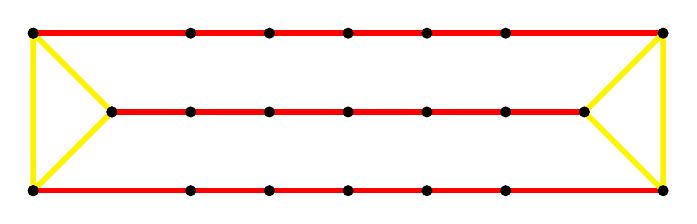
\begin{tikzpicture}
        \draw[yellow] (0,0) \kant (1,1) \kant (0,2) \kant cycle;
        \draw[red] (0,0) \kant (2,0);
        \draw[red] (2,0) \kant (3,0);
        \draw[red] (3,0) \kant (4,0);
        \draw[red] (4,0) \kant (5,0);
        \draw[red] (5,0) \kant (6,0);
        \draw[red] (6,0) \kant (8,0);
        \draw[red] (1,1) \kant (2,1);
        \draw[red] (2,1) \kant (3,1);
        \draw[red] (3,1) \kant (4,1);
        \draw[red] (4,1) \kant (5,1);
        \draw[red] (5,1) \kant (6,1);
        \draw[red] (6,1) \kant (7,1);
        \draw[red] (0,2) \kant (2,2);
        \draw[red] (2,2) \kant (3,2);
        \draw[red] (3,2) \kant (4,2);
        \draw[red] (4,2) \kant (5,2);
        \draw[red] (5,2) \kant (6,2);
        \draw[red] (6,2) \kant (8,2);
        \draw[yellow] (8,0) \kant (7,1) \kant (8,2) \kant cycle;
    \end{tikzpicture}
    \caption{The envelope example}\label{fig:envelope}
    % envelope example
    % red x_e = 1, yellow x_e = 1/2
    % LP = n
    % OPT = 4/3n - 2
\end{figure}

\begin{definition}[Integrality gap]
    The integrality gap of an linear program is defined as
    \begin{align*}
        \sup_{\text{instance I}} \frac{\OPT(I)}{\LP(I)}\;,
    \end{align*}
    where $\LP(I)$ is the optimal fractional and $\OPT(I)$ is the optimal integral solution.
\end{definition}

\begin{prop}
    The integrality gap of the subtour LP for instances satisfying the triangle inequality is at least $\frac43$.
\end{prop}
\begin{proof}
    Consider the graph in Figure~\ref{fig:envelope}.
    We set $x_e=1$ on the red edges and $x_e=0.5$ on the yellow ones.
    One can check that this a solution of the subtour LP with cost $|V|$.
    Now we try to find an optimal tour in the graph.
    We have to use at least $|V|$ edges for a cycle visiting $|V|$ nodes. 
    But we also need to use one of the red paths twice to be Eulerian.
    This adds $|V|/3 -2$ edges.
    So an optimal tour has at least length $4/3|V| - 2$.
\end{proof}


\begin{thm}[Spanning tree polytope (Edmonds)]\label{thm:mstpoly}
    The \emph{spanning tree polytope} of an undirected graph $G$, the convex hull of the incidence vectors of the edge sets of spanning trees in $G$, is
    \begin{align*}
        \left\{x\in \IR^{E(G)} \such x(E(G)) = n-1,~ x(E[U]) \leq |U|-1 ~( \emptyset\neq U\subsetneq V(G)),~ x\geq 0\right\}
    \end{align*}
\end{thm}

\begin{cor}
    For every vector $x$ in the subtour polytope, $\frac{n-1}nx$ is in the spanning tree polytope.
\end{cor}
\begin{proof}
    Let $x$ be in the subtour polytope. Then
    \begin{align*}
        \frac{n-1}n x(E) = \frac{n-1}{2n} \sum_{v\in V} x(\delta(v)) = n-1
    \end{align*}
    Let $\emptyset \neq U\subsetneq V$. 
    \begin{align*}
        x(E[U]) = \frac12 \left(\sum_{u\in U} x(\delta(u)) - x(\delta(U))\right) \leq \frac 12 (2|U| - 2) = |U| -1 
    \end{align*}
\end{proof}

Let $(V,S)$ be a minimum spanning tree. 
Then
\begin{align*}
    c(S) = \min\left\{c(x)\such x \text{ is in the spanning tree polytope}\right\} \leq c(x^*) = \LP
\end{align*}
where $x^*$ is an optimal solution to the subtour LP.

%% Thursday: c(J) <= 1/2 c(x*), together -> christofides <= 3/2 LP


\end{document}
